% !TEX root = ../sethomas_thesis_main.tex

\chapter{Designing Integrated Control Systems}
% Here, in this chapter, a novel control mechanical control strategy and SMA actuator is showcased and studied.

% Goal : Present the principle of integrated control systems in SMA Actuators
% Problem : Most SMA actuators require advanced control systems and complex control strategies to create actuators. This results in mechanisms that are less spatially efficient
% Solution : By integrating the SME and its mechanical connection to temperature into the control structure, this dependence can be exploited to create a novel control solution

\section{Introduction}
% Present different control structures : sensors and sensorless
Shape Memory Alloys, often referred to as artificial muscles, are often used in applications where a compact and lightweight solution is required. When paired with a biasing element such as a spring or compliant mechanism, a lightweight reversible actuator can be fabricated. By heating and cooling the active SMA element, a reversible back and forth motion can be created.

Due to the complex nature of the shape memory effect, sensors or complex control strategies are required for the accurate control of the SMA element, as shown in the work by \todocite and \todocite. The SMA, if overheated, can result in the permanent reprogramming of the shape or the destruction of the SMA wire or coil. In the case of smaller, more compact applications, the SMA element used are thin wires or coil. In these cases, using sensors that can measure the temperature can be quite difficult to implement due to the low thermal mass of the SMA element. Recent work such as \todocite, have implemented sensorless systems where the change in resistivity is measure as the SMA changes phase to create more compact control solutions. Here, due to the complex nonlinear nature of the shape memory effect requires complex control strategies and micro-controllers to efficiently control the SMA and prevent overheating.

Often, when considering the volumetric work density of SMA actuators, the electronics, sensors and control strategies are not taken into account. In certain applications, for example untethered crawling robots, the control plays an important role in the final work-weight density of the robot as seen in the work by \todocite. Improvements made in the sensorless and control strategies can, thus, have a major impact in the final dimensions and weight of the SMA actuator.

In this chapter, a novel design concept is presented to further integrate the discrete building blocks present in the traditional SMA actuator. By exploiting the dependence of the mechanical behaviour of the SMA and its temperature, a mechanical oscillator system can be developed such that an electronics-free SMA actuator can be designed. This design language can be implemented into SMA actuators to create a simple but effective solution to create a sensorless, micro-controller-free control strategy that intrinsically present SMA overheating. Furthermore, in this chapter, a crawling robot is conceived using this methodology to validate this novel design approach.

\section{Design Methodology for the Control System}
% Concept and working principle
As mentioned previously, due to the complex behaviour of SMAs, the sensors and control strategies required to actuate an SMA actuator can be cumbersome and reduce the overall work-weight density of the resulting robotic systems. The shape memory effect and the corresponding phase transitions are directly dependant on the temperature of the alloy. By exploiting this mechanical relationship between the temperature of SMA, the control system can be integrated into the kinematic stage, as represented in \todocite.
% Building blocks figure
\subsection{Working principle}
% example of similar solutions (or primitive tries)

A basic linear SMA actuator consists of an SMA and a biasing spring that when heated and cooled, results in a simple back forth oscillating motion. By accurately controlling the temperature of the SMA above its transition temperature and below a critical overheating temperature, the SMA can be made to provide a reliable actuation. This reversible actuation results in a back and forth mechanical movement of the biasing spring and the cyclical movement of the kinematic stage, if any. The basic concept of this methodology consists of tying the mechanical behaviour of the actuator into the control.

The SMA element in most cases is heating using Joule's heating by simply passing a current through the SMA and allowing the internal resistance of the SMA element to heat up by Joule's losses as shown in the work by \todocite. The cooling of the SMA generally consists of passively extracting the heat from the active element using natural convection with the cooler surrounding air. This simple strategy is often used in the control of SMA actuators due to not requiring any additional mechanisms and thus, does not reduce the work-density of the actuator while keeping the system compact.

Thus, by using the mechanical behaviour of the actuator to cut the current flow across the SMA will immediately cool the active element before it has a chance to overheat. In this manner, the control of the SMA actuator is mechanical controlled by the shape memory effect. Here, as a current is passed through the SMA wire or coil, it heats up the SMA resulting in a strain recovery and the SMA returning to its original length. This change in length, after a certain threshold, can be made to physically cut the electrical contact between the SMA element and the power supply. This cause the immediate cooling of the SMA through heat exchange with the surrounding air. As the SMA cools down, the biasing element will, once again, deform the SMA which will re-establish the electrical contact across the SMA, restarting the oscillating motion. Thus, this design strategy when integrated into the kinematic stage can render the entire SMA actuator compact and electronics-free.

% Advantages (maybe examples)
This approach, when properly implemented, can result in an robotic system where a reversible actuation can be observed without the need for any electronics, micro-controllers or sensors, preserving the work-weight density of the system. A mechanical control of the SMA element can result in a system where the SMA element, due to the physical electrical contacts being interrupted, can never overheat.

\subsection{Implementation}
% Implementation
% Bias spring using flexural linear stage
As mentioned earlier, using a flexure based mechanism as a linear guide, permits the omission of a dedicated spring in the design. As seen in \cref{fig:proto-closeup}, the linear stage is comprised of two parallel cantilever beams. These cantilevers act as leaf springs that apply a tractional return force on the SMA coil at a lower temperature while also preventing any unwanted degrees of freedom in the other axis.

The implementation of the oscillator mechanism consists of pairing the SMA actuator with a magnetic latch system. A diagram of the working principle of the prototype can be seen in \cref{fig:oscillator-schematic}. The magnetic latch consists of a magnet mounted on a leaf spring that is attracted to the free end of the SMA actuator. The electrical current is made to flow across the magnetic latch and into the SMA coil. Thus, the coil is only heated when the magnet makes contact with the free end of the actuator. Essentially, as the magnet connects to the actuator, the coil is heated and retracts. As the coil retracts, the magnet mounted on the leaf spring is displaced with the coil. During this phase, the magnet experiences a return force, $F_\textrm{S}$, and will continue to follow the actuator. Once, the return force is higher than the attractive magnetic force, $F_\textrm{mag}$, between the magnet and the SMA coil, the latch detaches immediately from the actuator and the magnet returns to its original location. This causes the electrical contact to be broken and begins the cooling of the SMA coil. The bias leaf spring of the SMA actuator will, in this phase, extend the coil back towards the magnetic latch to, once again, re-establish the electrical contact. In this manner, an oscillating behaviour can be observed without any control logic or sensors. Therefore, the required contraction of the SMA coil, $\varepsilon$, can be controlled by sizing the leaf spring associated with the magnet.
\begin{equation}\label{eq:sma-contraction}
    \varepsilon = \frac{F_\textrm{mag}}{K_s}
\end{equation}
where $K_s$ is the rigidity of the leaf spring which depends on the dimensions of the cantilever beams and can be calculated using \cite{henein-2017, howell_handbook_2013}.

This basic concept can be implemented using different methods. The linear stages can be further optimised and size to fit the desired stroke of the actuator. Solutions involving mechanical latches and pogo pins can be imagined to serve the same purpose.

\begin{figure}[ht] % t for top of the page, H could be put to impose the position of the float
  \centering
  \resizebox{0.6\textwidth}{!}{\input{images/chap6/proto-schematic.eps_tex}}
  \caption{Diagram showing the working principle of the magnetic latch system implemented in the SMA oscillator.}
  \label{fig:oscillator-schematic}
\end{figure}

\begin{figure}[ht] % t for top of the page, H could be put to impose the position of the float
  \centering
  \begin{tikzpicture}
    \begin{scope}[x={(graph.south east)},y={(graph.north west)}]
        \node[anchor=south west,inner sep=0] (image) at (0,0) {\includegraphics[width=0.75\textwidth]{images/chap6/proto-full.jpg}};
    \end{scope}
  \end{tikzpicture}%
  \caption{The integrated SMA control system implemented using a flexure-based magnetic latch creating an SMA mechanical oscillator.}
  \label{fig:proto-full}
\end{figure}

\begin{figure}[ht] % t for top of the page, H could be put to impose the position of the float
  \centering
  \begin{annotationimage}{trim={0 0cm 0 20cm},clip, width=0.75\textwidth}{images/chap6/proto-closeup.jpg}
   \draw[annotation right = {SMA Coil at 0.6}] to (0.85,0.48);
   \draw[annotation left = {Magnet at 0.6}] to (0.47,0.5);
   \draw[coordinate label = {Bias Leaf Spring at (0.74,0.1)}];
   \draw[coordinate label = {Leaf Spring at (0.27,0.1)}];
 \end{annotationimage}
  \caption{The close-up structure of the magnetic latch system that acts as the oscillating electrical contact for the SMA coil. Here, the biasing leaf spring also act as a linear stage for the actuator.}
  \label{fig:proto-closeup}
\end{figure}

% % Attempt at overpic osc prototype
% \begin{figure}[t]
%     \begin{tikzpicture}
%         \node[anchor=south west,inner sep=0] (graph) at (0,0) {
%         \begin{overpic}[trim={0 0cm 0 20cm},clip,width=0.45\textwidth]{
%             \begin{scope}[xshift=1.5cm]
%                 \node[anchor=south west,inner sep=0] (image) at (0,0) {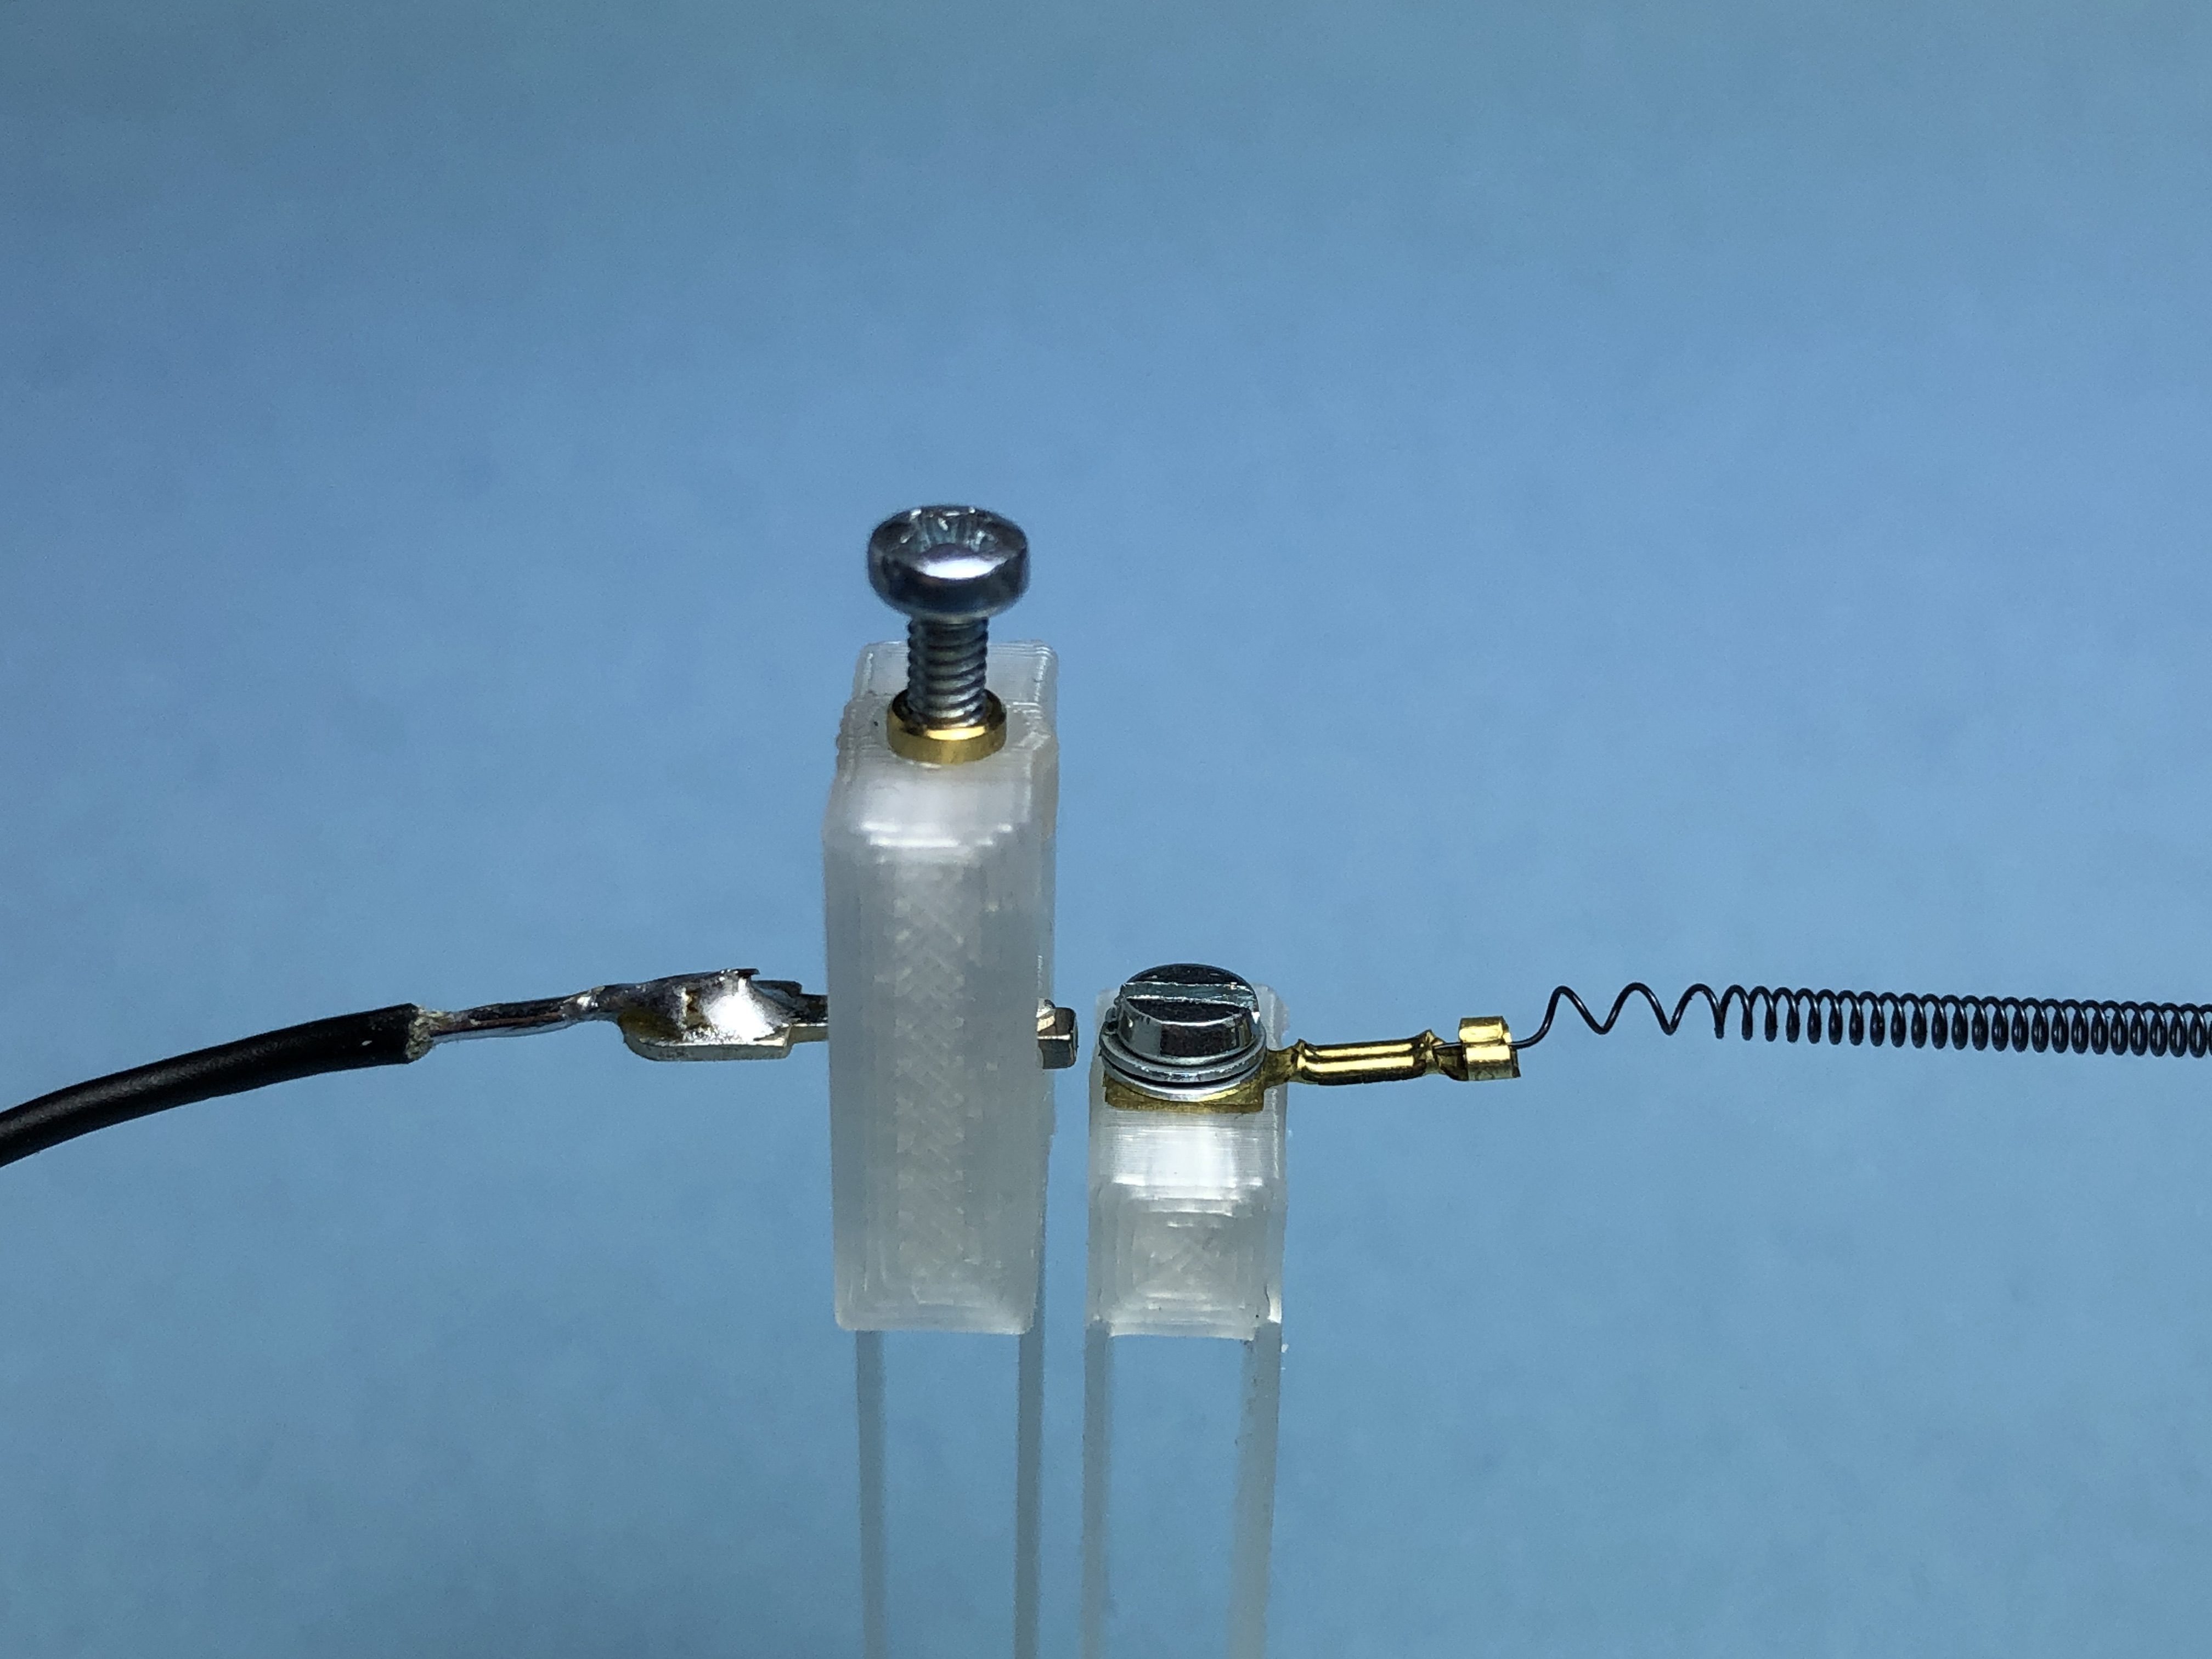
\includegraphics[trim={0 0cm 0 20cm},clip, width=0.45\textwidth]{images/chap6/proto-closeup.jpg}};
%                 \node [anchor=west] (magnettext) at (4.5,4) {\color{white} Magnet};
%                 \node [anchor=west] (SMA) at (6.9,2.9) {\color{white} \large SMA};
%                 \node [anchor=west] (BLS) at (4.8,0.3) {\color{white} Bias Leaf Spring};
%                 \node [anchor=east] (LS) at (3.1,0.3) {\color{white} Leaf Spring};
%                 % \node [anchor=east] (magnet) at (4.15,2.55);
%                 % \draw[->] (magnettext) edge (magnet)
%                 % \begin{scope}[x={(image.south east)},y={(image.north west)}]
%                 %     \draw[red,ultra thick,rounded corners] (0.48,0.80) rectangle (0.55,0.95);
%                 \draw [-latex, ultra thick, white] (magnettext) to (4,2.55);
%                 % \end{scope}
%             \end{scope}
%         }
%             \put(37,1){\color{white}\linethickness{0.3mm}% Zoomed image
%             \frame{\includegraphics[trim={0cm 0cm 0cm 0cm},clip,width=0.6\columnwidth]{figures/proto-full.jpg}}}
%         \end{overpic}
%         };
%      \end{tikzpicture}
%     \caption{The proof of concept of the magnetic latch system that acts as the oscillating electrical contact for the SMA coil. Here, the leaf spring also act as a linear stage for the actuator.}
%     \label{fig:proto-closeup}
% \end{figure}

% The SMA is supplied by \textit{Dynalloy, Inc} (Irvine, CA) and is a 90\degreeC Flexinol\textsuperscript{\textregistered} coil with wire diameter of 200 $\mu$m and an outer diameter of 1.4 mm. The coil contains around 40 coils and with a solid length of 8 mm. The SMA is mounted on a 3D printed support containing a flexure-based linear stage which supports the free end of the SMA. The linear stage is 3D printed from PLA and consists of 2 parallel leaf springs with dimensions 500 $\mu$m x 10 mm x 30 mm.

% Sizing strategies (thermal model) + results
\section{Validation of the Approach}
% Validation of the approach using a case study (introduction)
% Concept and motivation
% Working Principle
% Analytical Model
% Results and comparison
\section{Summary and Conclusion}
